\documentclass[a4paper]{article}
\usepackage[a4paper,margin=0mm]{geometry}
\usepackage{fontspec}
\usepackage{unicode-math}
\usepackage{tikz}
\usepackage[table]{xcolor}
\usepackage[absolute]{textpos}
\usepackage{enumitem}
\usepackage{array}
\usepackage{multirow}

\setmainfont{Libertinus Serif}
\setsansfont{Libertinus Sans}
\setmathfont{Libertinus Math}
\newfontfamily\trackedsans{Libertinus Sans}[LetterSpace=8.0]

\definecolor{accent}{HTML}{602785}
\definecolor{badge}{HTML}{B8A0C8}
\definecolor{ink}{HTML}{2A2E30}

\setlength{\TPHorizModule}{1mm}
\setlength{\TPVertModule}{1mm}
\setlength{\parindent}{0pt}
\pagestyle{empty}

% ---- Safe print margins: 16mm outer on both sides so bound/trimmed copies never
% clip problem text. Columns are 83mm wide with a 6mm gap on each side of the
% center rule (at x=105mm). ----
\newcommand{\LCOL}{16mm}
\newcommand{\RCOL}{111mm}
\newcommand{\COLW}{83mm}

% ---- Plain topic header: number chip + title, thin rule underneath. No band, no watermark. ----
\newcommand{\topicheader}[2]{%
\begin{textblock*}{194mm}(16mm,10mm)
\begin{tikzpicture}
\node[fill=accent,text=white,font=\sffamily\bfseries\fontsize{13}{13}\selectfont,
      minimum width=9mm,minimum height=9mm,inner sep=0pt] at (4.5mm,-4.5mm) {#1};
\node[font=\sffamily\bfseries\fontsize{15}{16}\selectfont,text=ink,anchor=west] at (12mm,-4.5mm) {#2};
\end{tikzpicture}
\end{textblock*}
\begin{textblock*}{194mm}(16mm,22.5mm)

\begin{tikzpicture}
\fill[accent] (0,0) rectangle (194mm,0.5mm);
\end{tikzpicture}
\end{textblock*}
}

\newcommand{\pagefooter}[1]{%
\begin{textblock*}{194mm}(8mm,286.41mm)
  
\begin{tikzpicture}
    \fill[accent] (0,0) rectangle (194mm,0.6mm);
  \end{tikzpicture}
\end{textblock*}
\begin{textblock*}{63.59mm}(8mm,288.27mm)
  {\sffamily\bfseries\color{accent}\fontsize{13}{16}\selectfont SAT 1200+}
\end{textblock*}
\begin{textblock*}{10mm}(188mm,288.27mm)
  \centering{\sffamily\color{accent}\fontsize{14}{16}\selectfont #1}
\end{textblock*}
}

% ---- Fixed-length vertical column rule: #1 = top y (mm), #2 = length (mm) ----
\newcommand{\colrule}[2]{%
\begin{textblock*}{1mm}(105mm,#1mm)
\begin{tikzpicture}
\draw[black!65,line width=0.5pt] (0,0) -- (0,#2mm);
\end{tikzpicture}
\end{textblock*}
}

\newcommand{\setkicker}[2]{%
{\sffamily\bfseries\fontsize{12}{14}\selectfont #1.}\ {\itshape\fontsize{10.3}{13}\selectfont\color{black!75} #2}\par\vspace{2mm}%
}

% ---- Small boxed problem number, reference-style. Plain \fbox -- stays flush with
% the text baseline instead of centering on it. ----
\setlength{\fboxsep}{1.4pt}
\setlength{\fboxrule}{0.5pt}
\newcommand{\pnum}[1]{\fcolorbox{ink}{white}{\sffamily\bfseries\fontsize{8}{8}\selectfont #1}~}

% ---- QR placeholder square + caption below ----
\newcommand{\qrbox}[1]{%
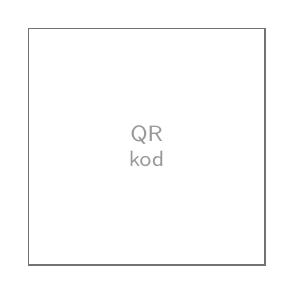
\begin{tikzpicture}
\draw[black!55,line width=0.6pt] (0,0) rectangle (30mm,30mm);
\node[black!40,font=\sffamily\fontsize{8}{9}\selectfont,align=center] at (15mm,15mm) {QR\\kod};
\end{tikzpicture}\\[1.5mm]
{\sffamily\fontsize{9}{11}\selectfont\color{black!70} #1}%
}

% ---- Answer-table styling: accent-colored grid ----
\arrayrulecolor{accent}
\setlength{\arrayrulewidth}{0.7pt}
\renewcommand{\arraystretch}{1.25}
\newcommand{\anstitle}[1]{{\sffamily\bfseries\color{accent}\fontsize{11}{13}\selectfont #1}\\[1.3mm]}

\begin{document}

% ================= PAGE 1: Set 1 | Set 2 =================
\topicheader{18}{Tadqiqot Dizayni va Statistik Xulosalar}
\pagefooter{1}
\colrule{32}{238}
\mbox{}%

\begin{textblock*}{\COLW}(\LCOL,32mm)
{\fontsize{10.3}{13}\selectfont
\setkicker{1-to'plam}{Tasodifiy tanlanmami yoki qulaylik tanlanmasi? Har bir holat uchun ayting va natijani umumlashtirish mumkinmi, tushuntiring.}

\noindent\pnum{1} Telefon ishlab chiqaruvchisi 400,000 ro'yxatdan o'tgan egalari ichidan kompyuter orqali tasodifiy tanlangan 2,000 mijozga so'rovnoma yuboradi.\\[14mm]
\noindent\pnum{2} Radio eshittirish tinglovchilarni yangi soliq qonuni haqida fikr bildirish uchun qo'ng'iroq qilishga chaqiradi; 300 kishi qo'ng'iroq qiladi.\\[14mm]
\noindent\pnum{3} Kasalxona o'tgan yili davolangan 10,000 bemorning to'liq bazasidan 150 ta fayl tasodifiy tanlab, o'rtacha tiklanish vaqtini o'rganadi.\\[14mm]
\noindent\pnum{4} Sport zali o'z Instagram sahifasida qaysi kunlarda mashq qilishni afzal ko'rishlari haqida so'rovnoma joylaydi; 600 obunachi javob beradi.\\[14mm]
\noindent\pnum{5} Milliy bog' qo'riqchisi parkka kiruvchi har 20-mashinani (ichida kim bo'lishidan qat'i nazar) to'xtatib, necha masofa bosib o'tganini so'raydi, toki 400 ta mashina so'rovdan o'tguncha.
}
\end{textblock*}

\begin{textblock*}{\COLW}(\RCOL,32mm)
{\fontsize{10.3}{13}\selectfont
\setkicker{2-to'plam}{Eksperimentmi yoki kuzatuv tadqiqotimi? Sabab-oqibat (causation) da'vo qilish mumkinmi yoki faqat bog'liqlik (correlation), ayting.}

\noindent\pnum{1} Tadqiqotchilar 80 ta o'simlikni tasodifiy ikki guruhga ajratadi: yangi o'g'it yoki oddiy suv, so'ng 3 haftadan keyin o'sishni o'lchaydi.\\[14mm]
\noindent\pnum{2} O'qituvchi old qatorda o'tiradigan o'quvchilarning test ballari orqa qatordagilarnikidan yuqoriroq ekanini payqaydi -- o'quvchilar o'zlari joy tanlagan.\\[14mm]
\noindent\pnum{3} Dorixona sinovi 300 ko'ngillini tasodifiy ikki guruhga ajratadi: yangi dori yoki platsebo, na ko'ngillilar, na shifokorlar qaysi guruh ekanini bilishmaydi.\\[14mm]
\noindent\pnum{4} Iqtisodchi 10 yillik milliy ma'lumotlarni o'rganib, muzqaymoq savdosi yuqori bo'lgan oylarda quyoshdan kuyish tashriflari ham yuqoriroq ekanini topadi.\\[14mm]
\noindent\pnum{5} Kompaniya xodimlarga uydan yoki ofisdan ishlashni o'zlari tanlashga ruxsat beradi, so'ng yil oxirida ikki (o'zi tanlagan) guruhning mahsuldorligini solishtiradi.
}
\end{textblock*}

\clearpage

% ================= PAGE 2: Set 3 | Set 4 =================
\topicheader{18}{Tadqiqot Dizayni va Statistik Xulosalar}
\pagefooter{2}
\colrule{32}{238}
\mbox{}%

\begin{textblock*}{\COLW}(\LCOL,32mm)
{\fontsize{10.3}{13}\selectfont
\setkicker{3-to'plam}{Aralash: tanlanma VA guruhlash birgalikda. Ikkalasi ham tasodifiymi, va aniq nima xulosa qilish mumkinligini ayting.}

\noindent\pnum{1} Universitet to'liq talabalar ro'yxatidan 500 nafarini tasodifiy tanlaydi, so'ng ularning yarmini yangi 15 daqiqalik kunlik usulga, yarmini odatdagi tartibga tasodifiy ajratadi, yakuniy imtihon ballarini o'lchaydi.\\[18mm]
\noindent\pnum{2} Fitnes blogerining 40 nafar obunachisi qadam-sanash tanlovi uchun o'z xohishi bilan ishtirok etadi; bloger ularning yarmini pedometr ilovasiga, yarmini esa unga tasodifiy ajratadi, o'rtacha kunlik qadamlarni solishtiradi.\\[18mm]
\noindent\pnum{3} Shahar kommunal to'lovlar bazasidan 1,000 xonadonni tasodifiy tanlaydi; xonadonlardan shunchaki quyosh panelidan foydalanadimi deb so'raladi va to'lovlar solishtiriladi.\\[18mm]
\noindent\pnum{4} 25 nafar psixologiya talabasidan iborat sinf (kattaroq populatsiyadan tasodifiy tanlanmagan) kuzatiladi: 8 soatdan ko'p uxlagan talabalar kam uxlaganlarga qaraganda test ballari yuqoriroq, hech qanday guruh tadqiqotchi tomonidan belgilanmagan.
}
\end{textblock*}

\begin{textblock*}{\COLW}(\RCOL,32mm)
{\fontsize{10.3}{13}\selectfont
\setkicker{4-to'plam}{Haddan oshishni toping. Qaysi qoida buzilganini (tanlanma, guruhlash yoki ikkalasi) ayting va to'g'ri ko'lamdagi xulosani qayta yozing.}

\noindent\pnum{1} Pazandachilik veb-sayti o'z axborot byulleteniga o'z xohishi bilan yozilgan 90 kishini so'raydi, 70 tasi yangi retseptni yoqtirganini topadi va da'vo qiladi: \textit{``Bu retsept hamma joyda uy oshpazlari orasida mashhur.''}\\[18mm]
\noindent\pnum{2} Tadqiqotchilar butun mamlakat bo'ylab tasodifiy tanlangan 200 kattalarni kunlik 10 daqiqalik meditatsiya guruhiga yoki meditatsiyasiz guruhga tasodifiy ajratadi va meditatsiya guruhida stress pastroq ekanini topadi. Blogger buni shunday yozadi: \textit{``Tadqiqotlar ko'rsatadiki, meditatsiya ba'zi odamlarni tinchlantiradi''} -- bu atayin noaniq ifoda, haqiqatda tadqiqot natijasini kamsitib ko'rsatayotganini baholang.\\[18mm]
\noindent\pnum{3} Milliy miqyosda tasodifiy tanlangan 2,000 kattalar o'rganiladi va zavq uchun muntazam o'qiydiganlarning xotira testi ballari yuqoriroq ekani topiladi. Gazeta sarlavhasi: \textit{``O'qish kattalarda xotirani yaxshilaydi.''}\\[18mm]
\noindent\pnum{4} Bitta maktab (tasodifiy tanlanmagan) o'z 120 nafar o'quvchisini yangi uy vazifasi ilovasi yoki eski qog'oz usuliga tasodifiy ajratadi, ilova guruhining baholari oshganini topadi. Tuman e'lon qiladi: \textit{``Bu ilova shtatdagi har bir o'quvchi uchun baholarni oshiradi.''}\\[18mm]
\noindent\pnum{5} Bitta savdo markazidagi 50 xaridor (hech qanday guruh belgilanmagan) kuzatiladi: sodiqlik ilovasidan foydalanganlar ko'proq xarajat qilgani topiladi. Marketing xati da'vo qiladi: \textit{``Bizning sodiqlik ilovamiz hamma joyda mijozlarni ko'proq xarajat qilishga majbur qiladi.''}
}
\end{textblock*}

\clearpage

% ================= PAGE 3: Set 5 | Set 6 (bonus) =================
\topicheader{18}{Tadqiqot Dizayni va Statistik Xulosalar}
\pagefooter{3}
\colrule{32}{238}
\mbox{}%

\begin{textblock*}{\COLW}(\LCOL,32mm)
{\fontsize{10.3}{13}\selectfont
\setkicker{5-to'plam}{To'g'ri xulosani yozing. Tadqiqot nimani qo'llab-quvvatlashi va nimani qo'llab-quvvatlay olmasligini o'z so'zlaringiz bilan yozing.}

\noindent\pnum{1} Milliy miqyosda tasodifiy tanlangan 600 kattalar (hech qanday guruh belgilanmagan) kofe iste'moli va o'zini qanday sezgani haqida so'raladi; kuniga 2+ chashka ichuvchilar o'zlarini sergakroq his qilishini aytishadi.\\[26mm]
\noindent\pnum{2} Biologiya laboratoriyasi (tasodifiy jalb qilinmagan, o'z xohishi bilan ishtirok etgan) 60 ta sichqonni yangi vitamin qo'shimchasi yoki nazorat ratsioniga tasodifiy ajratadi, qo'shimcha guruhida 8 haftadan keyin suyak zichligi yaxshiroq ekanini topadi.\\[26mm]
\noindent\pnum{3} Milliy miqyosda tasodifiy tanlangan 1,200 o'rta maktab o'quvchisi musiqa asbobida chalish va standartlashtirilgan test ballari haqida so'raladi; chaluvchilar o'rtacha yuqoriroq ball oladi, hech qanday guruh belgilanmagan.
}
\end{textblock*}

\begin{textblock*}{\COLW}(\RCOL,32mm)
{\fontsize{10.3}{13}\selectfont
\setkicker{6-to'plam}{Bonus / qiyin -- qatlamli holatlar. Har birida haqiqiy dizaynni aniqlang va xulosa asoslanganmi, tushuntiring.}

\noindent\pnum{1} Universitet 800 talabani ro'yxatidan tasodifiy tanlab, ularni yarim kunlik ish va GPA haqida so'raydi -- lekin 800 tadan faqat 110 tasi (o'z xohishi bilan) javob beradi. Universitet bu natija ``odatiy talaba''ni ifodalaydi, deb xulosa qiladi. Haqiqiy dizayn qanday va xulosa asoslanganmi?\\[26mm]
\noindent\pnum{2} Milliy miqyosda vakillik qiluvchi tasodifiy tanlangan 3,000 kattalar uyqu tadqiqotiga jalb qilinadi. Shu tanlanma ichida tadqiqotchilar yarmini yangi uyqu kuzatuv qurilmasiga, yarmini qog'oz kundaligiga tasodifiy ajratadi, qurilma guruhida uyqu jadvali barqarorroq ekanini topadi. Bu yerda mamlakat miqyosida sabab-oqibat da'vosi asoslanganmi va bu holat yuqoridagilardan nimasi bilan farq qiladi?\\[26mm]
\noindent\pnum{3} Qiyin holat: shirinlik kompaniyasi o'z ilova foydalanuvchilaridan (umumiy aholidan emas, balki o'z foydalanuvchi bazasidan) 500 nafarini tasodifiy tanlaydi va ularni yangi ta'm yoki klassik ta'mga tasodifiy ajratadi, yangi ta'm yuqoriroq baholanganini topadi. Kompaniya: ``Ilova foydalanuvchilarimiz orasida yangi ta'm afzal ko'riladi, lekin ilovamizdan hech qachon foydalanmaganlar uchun bu to'g'rimi, hali ayta olmaymiz'' deydi. Bu tor va aniq da'vo, boshqa holatlardan farqli o'laroq, asoslanganmi?
}
\end{textblock*}

\clearpage

% ================= PAGE 4: Javoblar -- Sets 1-3 =================
\topicheader{18}{Tadqiqot Dizayni va Statistik Xulosalar}
\pagefooter{4}
\mbox{}%

\begin{textblock*}{194mm}(16mm,30mm)
{\bfseries\itshape\color{accent}\fontsize{19}{21}\selectfont\centering Javoblar\par}
\end{textblock*}

\begin{textblock*}{194mm}(16mm,42mm)
{\fontsize{9.3}{11.5}\selectfont
\centering
\begin{tabular}{|>{\centering\arraybackslash}p{24mm}|>{\centering\arraybackslash}p{8mm}|p{138mm}|}
\hline
\rowcolor{badge!55}\textbf{To'plam} & \textbf{\#} & \textbf{Izoh}\\
\hline
\multirow{5}{24mm}{\centering 1-to'plam} & 1 & Tasodifiy -- har bir egada tanlanish imkoniyati teng, 400,000 ga umumlashtirsa bo'ladi.\\\cline{2-3}
 & 2 & Qulaylik/o'z xohishi -- faqat qo'ng'iroq qilganlar vakil, umumlashtirib bo'lmaydi.\\\cline{2-3}
 & 3 & Tasodifiy -- to'liq bazadan tanlangan, barcha bemorlarga umumlashtiriladi.\\\cline{2-3}
 & 4 & Qulaylik/o'z xohishi -- faqat javob bergan Instagram obunachilari, umumlashtirib bo'lmaydi.\\\cline{2-3}
 & 5 & Tasodifiy -- har 20-mashina tizimli tanlov, tashrif davridagi barcha tashrifchilarga umumlashtiriladi.\\\hline
\multirow{5}{24mm}{\centering 2-to'plam} & 1 & Eksperiment -- sabab-oqibat da'vo qilish mumkin (o'g'it o'sishga sabab bo'ldi).\\\cline{2-3}
 & 2 & Kuzatuv -- faqat bog'liqlik; joy tasodifiy belgilanmagan, boshqa omillar sabab bo'lishi mumkin.\\\cline{2-3}
 & 3 & Eksperiment -- sabab-oqibat da'vo qilish mumkin (shu sinov populatsiyasida).\\\cline{2-3}
 & 4 & Kuzatuv -- faqat bog'liqlik; yashirin omil (issiq ob-havo) ikkalasiga ham sabab.\\\cline{2-3}
 & 5 & Kuzatuv -- faqat bog'liqlik; xodimlar joyni o'zi tanlagan, boshqa farqlar sabab bo'lishi mumkin.\\\hline
\multirow{4}{24mm}{\centering 3-to'plam} & 1 & Tasodifiy tanlanma + tasodifiy guruhlash -- eng kuchli holat: sabab-oqibat ham, umumlashtirish ham mumkin.\\\cline{2-3}
 & 2 & Tasodifiy emas tanlanma (o'z xohishi) + tasodifiy guruhlash -- sabab-oqibat faqat shu 40 obunachi uchun, umumlashtirib bo'lmaydi.\\\cline{2-3}
 & 3 & Tasodifiy tanlanma + tasodifiy emas guruhlash (o'zlari tanlagan) -- faqat bog'liqlik, lekin shahar xonadonlariga umumlashtiriladi.\\\cline{2-3}
 & 4 & Tasodifiy emas tanlanma + tasodifiy emas guruhlash -- eng zaif holat: faqat shu sinf ichida bog'liqlik, umumlashtirib bo'lmaydi, sabab-oqibat yo'q.\\\hline
\end{tabular}
}
\end{textblock*}

\clearpage

% ================= PAGE 5: Javoblar -- Sets 4-6 + QR =================
\topicheader{18}{Tadqiqot Dizayni va Statistik Xulosalar}
\pagefooter{5}
\mbox{}%

\begin{textblock*}{194mm}(16mm,22mm)
{\fontsize{9.3}{11.5}\selectfont
\centering
\begin{tabular}{|>{\centering\arraybackslash}p{24mm}|>{\centering\arraybackslash}p{8mm}|p{138mm}|}
\hline
\rowcolor{badge!55}\textbf{To'plam} & \textbf{\#} & \textbf{Izoh}\\
\hline
\multirow{5}{24mm}{\centering 4-to'plam} & 1 & Tanlanma buzilgan -- o'z xohishi bilan yozilganlar, ``hamma joyda'' emas. To'g'ri: ``90 ko'ngillidan ko'pchiligi retseptni yoqtirdi.''\\\cline{2-3}
 & 2 & Hech qanday qoida buzilmagan -- aslida ifoda tadqiqot natijasini kamsitib ko'rsatadi (tasodifiy tanlanma + tasodifiy guruhlash to'liq umumlashtiriladigan sabab-oqibat xulosani qo'llab-quvvatlaydi); bu har bir xulosa haddan oshmasligini, ba'zilari ehtiyotkor bo'lishini ko'rsatadi.\\\cline{2-3}
 & 3 & Guruhlash buzilgan -- bu kuzatuv tadqiqoti, faqat bog'liqlik. To'g'ri: ``Zavq uchun o'qish kattalarda yaxshiroq xotira bilan bog'liq.''\\\cline{2-3}
 & 4 & Tanlanma buzilgan -- sabab-oqibat shu 120 o'quvchi uchun to'g'ri, lekin maktab o'zi tasodifiy tanlanmagan, shtat miqyosida umumlashtirib bo'lmaydi.\\\cline{2-3}
 & 5 & Ikkala qoida ham buzilgan -- qulaylik tanlanmasi (``hamma joyda'' emas) va tasodifiy guruhlash yo'q (o'zlari tanlagan), faqat shu savdo markazida ham faqat bog'liqlik.\\\hline
\multirow{3}{24mm}{\centering 5-to'plam} & 1 & Qo'llab-quvvatlaydi: kofe va sergaklik orasidagi bog'liqlik, kattalarga umumlashtiriladi. Qo'llab-quvvatlamaydi: kofe sergaklikka sabab bo'lishini (guruhlash yo'q).\\\cline{2-3}
 & 2 & Qo'llab-quvvatlaydi: qo'shimcha suyak zichligiga sabab bo'lishini, lekin faqat shu sichqonlar populatsiyasi uchun. Qo'llab-quvvatlamaydi: barcha sichqonlar yoki turlarga umumlashtirishni.\\\cline{2-3}
 & 3 & Qo'llab-quvvatlaydi: asbob chalish va yuqori ball orasidagi bog'liqlik, o'quvchilarga umumlashtiriladi. Qo'llab-quvvatlamaydi: asbob chalish ballarga sabab bo'lishini (guruhlash yo'q).\\\hline
\multirow{3}{24mm}{\centering 6-to'plam} & 1 & Haqiqiy dizayn zaifroq: 800 tasodifiy tanlangan, lekin faqat 110 tasi o'z xohishi bilan javob bergan (javobsizlik muammosi) -- ``odatiy talaba'' xulosasi to'liq asoslanmagan.\\\cline{2-3}
 & 2 & Ha -- mamlakat miqyosida sabab-oqibat asoslangan, chunki ikkala shart ham bajarilgan: tasodifiy vakillik tanlanma VA tasodifiy guruhlash. Boshqa ko'p holatlar faqat bittasini qondiradi.\\\cline{2-3}
 & 3 & Ha -- bu tor da'vo to'liq asoslangan: tanlanma tasodifiy, lekin faqat kompaniya foydalanuvchilaridan; kompaniya da'vo ko'lamini aynan tanlanma ko'lamiga mos qiladi.\\\hline
\end{tabular}
}
\end{textblock*}

\begin{textblock*}{194mm}(16mm,243mm)
\centering
{\sffamily\fontsize{9.5}{11.5}\selectfont\color{black!70} Video yechimlar va qo'shimcha testlar uchun quyidagi QR kodlarni skanerlang:}\\[4mm]
\begin{minipage}[t]{32mm}\centering\qrbox{YouTube}\end{minipage}%
\hspace{16mm}%
\begin{minipage}[t]{32mm}\centering\qrbox{Telegram}\end{minipage}
\end{textblock*}

\end{document}
